
\documentclass[11pt]{report}
\usepackage{makeidx}
\usepackage{url}
\usepackage{a4wide}
\usepackage{longtable}
\usepackage{alltt,xspace}
\usepackage{hyperref}
\usepackage{subfigure,graphicx,epsfig,epsf,amsmath,amsfonts,float}


\parskip5pt
\makeindex 
\parindent0pt
\sloppy 
\begin{document}
\newcommand{\FLORA}{{\mbox{\sc ${\cal F}${lora}\rm\emph{-2}}}\xspace}
\newcommand{\fl}{F-logic }

\newcommand{\fd}{{\mbox{\tt \,->\,}}}                   % scalar
\newcommand{\bfd}{{\mbox{\tt \,*->\,}}}            % " + inheritable
\newcommand{\mvd}{{\mbox{\tt \,->\,}}}  % multivalued
\newcommand{\bmvd}{{\mbox{\tt \,*->\,}}}              % " + inheritable
\newcommand{\Fd}{{\mbox{\tt \,=>\,}}}                      % scalar signature
\newcommand{\Mvd}{{\mbox{\tt \,=>\,}}}  % multivalued signature
\newcommand{\bFd}{{\mbox{\tt \,*=>\,}}}                      % scalar signature
\newcommand{\bMvd}{{\mbox{\tt \,*=>\,}}}  % multivalued signature
\newcommand{\thismodule}{{\tt \_@}\xspace}

\def\Protege{Prot\'{e}g\'{e} }
\def\NoProtege{Prot\'{e}g\'{e}}

\title{\bf A Guide to \FLORA Packages
        \vspace{0.7cm}\\
 
\includegraphics[width=1in]{floralogo} 
           \vspace{3mm}\\
       {\Large Version 0.99.4}
       \\
       {\large (Kumquat)}
}


\maketitle


\thispagestyle{empty}
\newpage
\thispagestyle{empty}

\pagenumbering{roman}
\tableofcontents
\newpage        % Just to avoid a silly LaTeX bug with \pagenumbering
  
\pagenumbering{arabic}

\chapter[Persistent Modules]{Persistent Modules\\{by Vishal Chowdhary}}



\newcommand{\psm}{\mbox{PM}\xspace}

This chapter describes a \FLORA package that enables persistent modules.  A
\emph{persistent module} (abbr., \psm) is like any other \FLORA module
except that it is associated with a database. Any insertion or deletion of
base facts in such a module results in a corresponding operation on the
associated database. This data persists across \FLORA sessions, so the data
that was present in such a module is restored when the system restarts and
the module is reloaded.
  

\section{PM Interface}

A module becomes persistent by executing a statement that associates the
module with an ODBC data source. To start using the module persistence
feature, first load the following package into some module. For instance:
%% 
\begin{verbatim}
  ?- [persistentmodules>>pm].
\end{verbatim}
%% 
The following API is available. Note that if you load {\tt
  persistentmodules} into some other module, say {\tt foo}, then {\tt foo}
should be used instead of {\tt pm}.    
%%
\begin{itemize}
\item {\tt ?- ?Module[attach(?DSN,?DB,?User,?Password)]@pm.}\\
  This action associates the data source described by an ODBC {\tt DSN}
  with the module.  If {\tt ?DB} is a variable then the database is taken
  from the DSN. If {\tt ?DB} is bound to an atomic string, then that particular
  database is used. Not all DBMSs support the operation of replacing the
  DSN's database at run time. For instance, MS Access or PostgresSQL do not.
  In this case, {\tt ?DB} must stay unbound or else an error will be issued.
  For other DBMS, such as MySQL, SQL Server, and Oracle, {\tt ?DB} can be
  bound. 

  The {\tt ?User} and {\tt ?Password} must be bound to the user name and
  the password to be used to connect to the database.

  The database specified by the DSN must already exist. Otherwise, an
  exception of the form {\tt
    FLORA\_ABORT(FLORA\_DB\_EXCEPTION(?ErrorMsg,?))} is thrown.  (In a
  program, include {\tt flora\_exceptions.flh} to define {\tt
    FLORA\_DB\_EXCEPTION}; in the shell, use the symbol {\tt
    '\_\$flora\_db\_error'}.)  The database used in the {\tt attach}
  statement must not be accessed directly---only through the persistent
  modules interface.  The above statement will create the necessary tables
  in the database, if they are not already present.

  Note that the same database can be associated with several different
  modules. The package will not mix up the facts that belong to different
  modules.
\item {\tt ?- ?Module[attachNew(?DSN,?DB,?User,?Password)]@pm.}\\
  Like {\tt attach}, but a new database is created as specified by {\tt
    ?DSN}.  If the same database already exists, an exception of the form
  {\tt FLORA\_DB\_EXCEPTION(?ErrorMsg)} is thrown.  (In a program, include
  {\tt flora\_exceptions.flh} to define {\tt FLORA\_DB\_EXCEPTION}; in the
  shell, use the symbol {\tt '\_\$flora\_db\_error'}.)  This method creates
  all the necessary tables, if they are not already present.
  
  Note that this command works only with database systems that understand
  the SQL command {\tt CREATE DATABASE}. For instance, MS Access does not
  support this command and will cause an error.
\item {\tt ?- ?Module[detach]@pm.}\\
  Detaches the module from its database. The module is no longer persistent
  in the sense that subsequent changes are not reflected in any database.
  However, the earlier data is not lost. It stays in the database and the
  module can be reattached to that database.
\item {\tt ?- ?Module[loadDB]@pm.}\\
  On re-associating a module with a database (i.e., when {\tt
    ?Module[attach(?DSN, ?DB,?User,?Password)]@pm} is called in a new
  \FLORA session), database facts previously associated with the module are
  loaded back into it.  However, since the database may be large, \FLORA
  does not preload it into the main memory. Instead, facts are loaded
  on-demand.  If it is desired to have all these facts in main
  memory at once, the user can execute the above command. If no previous
  association between the module and a database is found, an exception is
  thrown.
\end{itemize}



Once a database is associated with the module, querying and insertion of
the data into the module is done as in the case of regular (transient)
modules.  Therefore \psm's provide a transparent and natural access to the
database and every query or update may, in principle, involve a database
operation.  For example, a query like {\tt ?- ?D[dept -> ped]@StonyBrook.}
may invoke the SQL {\tt SELECT} operation if module {\tt StonyBrook} is
associated with a database.  Similarly {\tt  insert\{a[b \fd
  c]@stonyBrook\}} and {\tt delete\{a[e \fd f]@stonyBrook\}}  will invoke
SQL {\tt INSERT} and {\tt DELETE} commands, respectively. Thus, \psm's provide
a high-level abstraction over the external database.

Note that if {\tt ?Module[loadDB]@pm} has been previously executed,
queries to a persistent module will \emph{not} access the database since
\FLORA will use its in-memory cache instead. However, insertion and
deletion of facts in such a module will still cause database operations.

\section{Examples}

Consider the following scenario sequence of operations.

%%
\begin{verbatim}
// Create new modules mod, db_mod1, db_mod2.
flora2 ?- newmodule{mod}, newmodule{db_mod1}, newmodule{db_mod2}.
flora2 ?- [persistentmodules>>pm].

// insert data into all three modules.
flora2 ?- insert{q(a)@mod,q(b)@mod,p(a,a)@mod}.
flora2 ?- insert{p(a,a)@db_mod1, p(a,b)@db_mod1}.
flora2 ?- insert{q(a)@db_mod2,q(b)@db_mod2,q(c)@db_mod2}.

//  Associate modules db_mod1, db_mod2 with an existing database db
//  The data source is described by the DSN mydb.
flora2 ?- db_mod1[attach(mydb,db,user,pwd)]@pm.
flora2 ?- db_mod2[attach(mydb,db,user,pwd)]@pm.

// insert more data into db_mod2 and mod.
flora2 ?- insert{a(p(a,b,c),d)@db_mod2}.
flora2 ?- insert{q(a)@mod,q(b)@mod,p(a,a)@mod}.

// shut down FLORA-2
flora2 ?- _halt.
\end{verbatim}
%%

\noindent
Restart the \FLORA system.

%%
\begin{verbatim}
// Create the same modules again
flora2 ?- newmodule{mod}, newmodule{db_mod1}, newmodule{db_mod2}.

// try to query the data in any of these modules.
flora2 ?- q(?X)@mod.
No.

flora2 ?- p(?X,?Y)@db_mod1.
No.

//  Attach the earlier database to db_mod1.
flora2 ?- [persistentmodules>>pm].
flora2 ?- db_mod1[attach(mydb,db,user,pwd)]@pm.

// try querying again...

// Module mod is still not associated with any database and nothing was
// inserted there even transiently, we have:
flora2 ?- q(?X)@mod.
No.

// But the following query retrieves data from the database associated
// with db_mod1.
flora2 ?- p(?X,?Y)@db_mod1.
?X = a,
?Y = a.

?X = a,
?Y = b.

Yes.

// Since db_mod2 was not re-attached to its database,
// it still has no data, and the query fails.
flora2 ?- q(?X)@db_mod2.

No.
\end{verbatim}
%%



%%% Local Variables: 
%%% mode: latex
%%% TeX-master: "flora-packages"
%%% End: 

\chapter[SGML and XML Parser for \FLORA]{SGML and XML Parsers for \FLORA\\ {by Rohan Shirwaikar}}



    This chapter documents the \FLORA package that provides SGML and
    XPath parsing capabilities. One set of predicates supports parsing
    SGML, XML, and HTML documents, which creates \FLORA objects in the user
    specified module. Other predicates evaluate XPath queries
    on XML documents and create \FLORA objects in user specified
    modules. The predicates make use of the {\bf sgml} and {\bf xpath}
    packages of XSB.
 


\section{Summary of the Predicates}

\begin{longtable}[l]{ll}
  {\bf load\_xml\_structure/3}&Parse XML data into \FLORA objects\\
  {\bf load\_sgml\_structure/3}&Parse SGML data into \FLORA objects\\
  {\bf load\_html\_structure/3}&Parse HTML data into \FLORA objects\\
  {\bf load\_xhtml\_structure/3}&Parse XHTML data into \FLORA objects\\
  {\bf parse\_xpath\_xml/3}&Apply an XPath expression to an XML
  document and parse the result\\
  {\bf parse\_xpath\_sgml/4}&Apply an XPath expression to an SGML
  document and parse the result\\
  {\bf parse\_xpath\_html/4}&Apply an XPath expression to an HTML document and parse the result\\
  {\bf parse\_xpath\_xhtml/4}&Apply an XPath expression to an XHTML document and parse the result\\
\end{longtable}

\section{Description}

This package supports parsing SGML, XML, and HTML documents,
converting them to sets of \FLORA objects stored in user-specified
\FLORA modules. The SGML interface
provides facilities to parse input in the form of files,
URLs and strings (Prolog atoms).  

For example, the following XML snippet

\begin{verbatim}
<greeting id='1'>
<first ssn=111'>
John
</first>
</greeting>
\end{verbatim}

will be converted into the following \FLORA objects:

\begin{verbatim}
o1[ element -> {o2}]
o2[ id = '1']
o2[ first -> {o3}]
o2[ ssn -> '111']
\end{verbatim}

To load the {\tt flrxml} package, the user should run the
following command at the \FLORA prompt.

%%
\begin{verbatim}
  flora?- [flrxml]. 
\end{verbatim}
%%

The following predicates are provided by the {\tt flrxml} package.  They
take SGML, XML, HTML, or XHTML documents and create the corresponding
\FLORA objects as specified in Section~\ref{xml-to-flora}.

\begin{description}
\item [load\_sgml\_structure({\tt +?Source,-?Warn,+?Module})@flrxml]
\item[load\_xml\_structure({\tt +?Source,-?Warn,+?Module})@flrxml]
\item[load\_html\_structure({\tt +?Source,-?Warn,+?Module})@flrxml]
\item[load\_xhtml\_structure({\tt +?Source,-?Warn,+?Module})@flrxml]
\end{description}
%%
The arguments to these predicates have the following meaning:

{\tt ?Source} is an input SGML, XML, HTML, or XHTML document.
It is of the form {\tt url({\tt {url}})},
{\tt file('{\tt {file name}}')} or {\tt string('{\tt document as a string}')}. 
{\tt ?Module} is the name of the \FLORA module where the objects created
by {\tt flrxml}  should be placed. {\tt ?Module}  must be bound.
{\tt ?Warn} gets bound to a list of warnings, if any are generated, or to
an empty list.
  

\section{XPath Support}

XPath support is based on the XSB {\tt xpath} package, which must be
configured as explained in the XSB manual. This package, in turn, relies on
the XML parser called {\tt libxml2}. It comes with most Linux
distributions and is also available for Windows, MacOS, and other
Unix-based systems from {\tt http://xmlsoft.org}. 
Note that both the library itself and the {\tt .h} files of that
library must be installed. 

The following predicates are provided. They select parts of the input
document using the provided XPath expression and create \FLORA objects as
specified in Section~\ref{xml-to-flora}. These predicates handle XML, SGML,
HTML, and XHTML, respectively.

\begin{description}
\item[parse\_xpath\_xml({\tt +?Source,+?XPath,+?NamespacePrefixList,-?Warn,+?Module})@flrxml]
\item[parse\_xpath\_sgml({\tt +?Source,+?XPath,+?NamespacePrefixList,-?Warn,+?Module})@flrxml]
\item[parse\_xpath\_html({\tt +?Source,+?XPath,+?NamespacePrefixList,-?Warn,+?Module})@flrxml]
\item[parse\_xpath\_xhtml({\tt +?Source,+?XPath,+?NamespacePrefixList,-?Warn,+?Module})@flrxml]
\end{description}
%%
The arguments have the following meaning:

{\tt Source} specifies the input document; this parameter has the same
format as in {\tt load\_structure}. {\tt ?XPath} is an XPath expression
specified as a Prolog atom. \emph{?Module} is the module where the resulting
\FLORA objects should be placed. {\tt ?Module} must be bound. \emph{?Warn}
gets bound to a list of warnings, if any are generated during the
processing, or to an empty list.

{\tt ?NamespacePrefixList} is a string that looks like a
space separated list of items of the form {\tt
  \emph{prefix} = \emph{namespaceURL}}. This allows one to use namespace
prefixes in the
XPath query given in the \emph{?XPath} parameter.
For example if the XPath expression is {\tt '/x:html/x:head/x:meta'}
where {\tt x} 
stands for {\tt 'http://www.w3.org/1999/xhtml'}, then this
prefix would have to be
defined in {\tt ?NamespacePrefixList}:

%%
\begin{verbatim}	
    parse_xpath_xhtml(url('http://w3.org'),
                      '/x:html/x:head/x:meta',
                      'x=http://www.w3.org/1999/xhtml',
                      ?Warnings,
                      foomodule)@flrxml.
\end{verbatim}
%%



\section{Mapping XML to \FLORA}\label{xml-to-flora}

This mapping is based on a proposal by Guizhen Yang.
It specifies how an XML parser can construct the
corresponding F-logic objects as a result of parsing an input XML
document.

The basic idea is as follows:
\begin{itemize}
\item Elements in XML are modeled as objects in F-logic.

\item Subelements in XML are modeled as multivalued attributes in F-logic.

\item Element attributes in XML are modeled as single-valued attributes
    in F-logic. This complies to the XML 1.0 specification which states
    that an attribute be defined only once for each element in an XML
    document.
\end{itemize}

This proposal deals with data-intensive XML documents, i.e., those that
don't rely on the interpretation of comments or processing instructions to
carry data. However, this proposal does consider the modeling of mixed
element content in which text and subelements are interspersed.

We do not consider modeling XML entities either, assuming no entity
references or that all entity references in the original XML document
are already resolved by an XML parser.



\subsection{Object Ids}

According to the XML specification 1.0, an XML element can be defined
with an oid that is unique across the document. Such an oid can be
provided as the value of an element attribute of type ID, although
this attribute can be arbitrarily named. Since an XML element is
modeled as an F-logic object, we would like the oid of this object to
take the value of any ID attribute if such value is defined.
Otherwise, the oid must be automatically generated by the system.

Sitting on top of the XML root element, there is an additional root
object which just functions as the access point to the entire object
hierarchy.

Note:
\begin{itemize}
\item Only a validating XML parser can decide whether an attribute
    is an ID attribute since such definition is provided by a DTD.

\item The oids of leaf nodes, which have no outgoing edges and carry
    plain text, are just the string values.
\end{itemize}

For example, the following XML document:

%%
\begin{verbatim}
<?xml version="1.0"?>
<person ssn="111-22-3333">
  <name first="John"                       (Example 1)
        last="Smith"/>
</person>
\end{verbatim}
%%
is represented by the following F-logic objects, provided we already
know that {\tt ssn}  is an ID attribute:
%%
\begin{verbatim}
   o1[person -> {'111-22-3333'}].
   '111-22-3333'[ssn -> '111-22-3333',
                 name -> {o2}
                ].
   o2[first -> 'John', last -> 'Smith'].
\end{verbatim}
%%


\subsection{Text and Mixed Element Content}

The content of an XML element may consist of plain text, or
subelements interspersed with plain text, for instance:

%%
\begin{verbatim}
  <greeting>Hi! My name is <first>John</first> <last>Smith</last>.</greeting> 
\end{verbatim}
%%

Each text segment is modeled in F-logic as if it were referred to by a
special tag, named {\tt '\$text'}.  Corresponding to each text segment, a node
is created and is referred to from the parent node by an edge labeled
{\tt '\$text'}. The text becomes the value of a special single-valued
attribute, named {\tt '\$string'},  of the newly created node. Moreover, if the
content of an XML element consists solely of plain text, then the text
also becomes the value of a special single-valued attribute of this
element, named {\tt '\$content'},  which is introduced for convenience purpose.

Therefore, the above XML segment would generate the following F-logic
objects, where {\tt o1, ..., o9}   are new oids:

\begin{verbatim}
o1[greeting -> {o2}].
o2['$text' -> {o3},
   first -> {o4},
   '$text' -> {o6},
   last  -> {o7},
   '$text' -> {o9}
  ].
o3['$string' -> 'Hi! My name is '].
o4['$content' -> 'John', '$text' -> {o5}].
o5['$string' -> 'John'].
o6['$string' -> ' '].
o7['$content' -> 'Smith', '$text' -> {o8}].
o8['$string' -> 'Smith'}.
o9['$string' -> '.'].
\end{verbatim}

Note:
\begin{itemize}
\item Handling of the whitespaces depends on the application. In the
  examples shown here, we assume that
  ``insignificant'' whitespaces have been omitted by the XML parser.
\item {\tt '\$content'}  can also be defined for every element. Its value is
    just the ASCII string as it appeared in the original document.
\end{itemize}

\subsection{Multivalued XML Attributes}

XML element attributes of type IDREFS are multivalued, in the sense
that their value is a string consisting of one or more oids separated
by whitespaces. Therefore, the value of such an attribute is a set. To
stick to the convention that element attributes are modeled as
single-valued attributes in F-logic, the value of an XML IDREFS
attribute is represented as a list.

For example, the following XML segment:
%%
\begin{verbatim}
<paper id="yk00" references="klw95 ckw91">
  <title>paper title</title>
</paper>
\end{verbatim}
%%
will generate the following F-logic atoms, assuming that the
{\tt reference}  attribute is of type IDREFS:
%%
\begin{verbatim}
yk00[references -> [klw95,ckw91],
       title -> {o1}
      ].
o1['$content' -> 'paper title', '$text' -> {o2}].
o2['$string' -> 'paper title'].
\end{verbatim}
%%
Note that since attribute definitions are provided by DTDs, only a
validating XML parser can decide whether an element attribute has the type
IDREFS.  A non-validating parser should just output the attribute values as
strings. The semantics of these strings is subject to further
interpretation by the applications.


\subsection{Ordering}

XML is order-sensitive, since XML DTDs impose order among elements.
For example, the following DTD element definition
%%
\begin{verbatim}
  <!ELEMENT book (author+, title, ISBN?)> 
\end{verbatim}
%%
states that the content of a {\tt book}  element consists of one or more
{\tt author}  element, followed by one {\tt title}  element, followed by an
optional {\tt ISBN}  element.
Note that XML 1.0 does not prescribe any order among element attributes.

Preserving the order of elements can also be useful for translating F-logic
objects back into an XML document.

A total order among the elements in an XML document should suffice to
establish the order in which the elements appear sequentially in the
XML document. In other words, such a total order should correspond to
the order in which the element open tags appear. In addition, the
ordering should also take into account the mixed element contents in
which each text segment is referred to by a {\tt '\$text'}  attribute.

\begin{verbatim}
<?xml version="1.0"?>
<person ssn="111-22-3333">
  <name>
    <first>John</first>                       (Example 2)
    <last>Smith</last>
  </name>
  <email>jsmith@abc.com</email>
</person>
\end{verbatim}


For example, the XML document in Example 2 can be represented by the
following tree, in which the integers enclosed by parentheses beside
the nodes represent the order assigned to the elements:

\begin{verbatim}
                    o1 (0)
                    |
                    | person
                    |
               '111-22-3333' (1)
                   / \
             name /   \ email
                 /     \
            (2) o2     o7 (7)
               / \       \ 
        first /   \last   \ '$text'
             /     \       \
        (3) o3     o5 (5)  o8 (8)
            |      |       'jsmith@abc.com'
    '$text' |      |'$text'
            |      |
        (4) o4     o6 (6)
           'John'  'Smith'
\end{verbatim}

Pre-order traversal of the XML tree will generate the total order for
the XML elements and text segments.

The ordering information that exists in XML documents is encoded as
follows. For each node, we introduce a special single-valued attribute,
named {\tt '\$order'}, which stores the order number.

\begin{verbatim}
<bibliography>
<paper id="sb97">
  <author>
    <first>John</first>
    <last>Smith</last>
  </author>
  <author>
    <first>David</first>
    <last>Brown</last>
  </author>                                  (Example 3)
</paper>

<paper id="s91">
  <author>
    <first>John</first>
    <last>Smith</last>
  </author>
</paper>
</bibliography>
\end{verbatim}


\subsection{More on Special Attributes}

The following special attributes are all single-valued.  Note that
this proposal does not intend to eliminate redundant information that
may exist across various attributes. It is up to the implementation to
decide whether to generate these attributes extensionally or
intentionally.

\begin{enumerate}
\item {\tt '\$tag'} \\
For each node, {\tt '\$tag'}  returns the unordered label of the edge
pointing to this node. {\tt '\$tag'}  can be defined as follows:
  %%
  \begin{verbatim}
     O['$tag' -> Tag] :- _[Tag -> {O}].
  \end{verbatim}
  %%
Note that for a node representing a text segment, the value of
its {\tt '\$tag'}  attribute is {\tt '\$text'}. 

\item {\tt '\$parent'} \\
For each node, {\tt '\$parent'}  returns the oid of the parent node.

\item {\tt '\$leftSibling'} \\
For each node, {\tt '\$leftSibling'}  returns the oid of the node appearing
immediately before the current node. This attribute is not defined
for the nodes without a left sibling.

\item {\tt '\$rightSibling'} \\
For each node, {\tt '\$rightSibling'}  returns the oid of the node appearing
immediately after the current node. This attribute is not defined
for those nodes without a right sibling.

\item {\tt '\$childrenNum'} \\
For each node, {\tt '\$childrenNum'}  returns the number of children including
nodes representing text segments.

\item {\tt '\$childrenList'} \\
For each node, {\tt '\$childrenList'}  returns a list, which is ordered, of the
oids of its children. Note that each text segment is also counted
as a child node.

\item {\tt '\$child'(N)} \\
For each node, {\tt '\$child'(N)} returns the {\tt N}-th child, where {\tt 1
  $\leq$ N} and {\tt N $\leq$ '\$chidlrenNum'}.

\item {\tt '\$tagList'} \\
For each node, {\tt '\$tagList'}  returns an ordered list of the
tags of its children. Note that each text segment is also counted
as if it were enclosed by a {\tt '\$text'}  tag.

\item {\tt '\$tag'(N)} \\
For each node, {\tt '\$tag'(N)}  returns the tag of the {\tt N}-th child, where {\tt 1
  $\leq$ N} and {\tt N $\leq$ '\$chidlrenNum'}.
This attribute can be defined as follows:

  %%
  \begin{verbatim}
     O['$tag'(N) -> Tag] :- O['$child'(N) -> V['$tag' -> Tag]]. 
  \end{verbatim}
  %%
\end{enumerate}

Note:
  The aforesaid attribute {\tt '\$content'}  can be defined
  for the nodes whose content is pure text as follows:

    %%
    \begin{verbatim}
      O['$content' -> String] :- 
	       O['$childrenNum' -> 1].text(1)['$string' -> String].
    \end{verbatim}
    %%

%%% Local Variables: 
%%% mode: latex
%%% TeX-master: "flora-packages"
%%% End: 



\chapter[JAVA Interface for \FLORA]{JAVA Interface for \FLORA\\by Aditi
      Pandit and Michael Kifer}


     This chapter documents the API for accessing \FLORA from a Java program.
  The API has two versions: a \emph{low-level API},
  which enables Java programs to
  send arbitrary queries to \FLORA and get results, and a \emph{high-level
    API}, which is more limited, but is easier to use. The high-level API
  establishes a correspondence between Java classes and \FLORA classes,
  which enables manipulation of \FLORA classes by executing appropriate
  methods on the corresponding Java classes. Both interfaces rely on the
  Java-XSB interface, called \emph{Interprolog}, provided by Declarativa.com.


\section{Description}
\subsection{The Low-level Interface}
 The low-level API enables Java programs to send arbitrary queries
to \FLORA and get results. 

In order to be able to access \FLORA, the Java program must first establish
a session for a running instance of \FLORA. Multiple sessions can be active
at the same time. The knowledge bases in the different running instances
are completely independent. Sessions are instances of
the class {\tt
javaAPI.src.FloraSession}. This class provides methods
for opening/closing sessions and loading \FLORA knowledge bases
(which are also used in the high-level
interface). In addition, a session provides 
methods for executing arbitrary \FLORA queries. The following is the complete
list of the methods that are available in that class.
\begin{itemize}
\item
\begin{verbatim}
public FloraSession()
\end{verbatim}
    This method creates a connection to an instance of \FLORA.
The initialization parameters needed are:

{\tt JAVA\_BIN}. This variable points to the directory containing
the javac and java executable programs. This variable is specified in
the {\tt windowsVariables.bat} and  {\tt unixVariables.sh}  files in the
{\tt java} subdirectory of the \FLORA distribution.

{\tt XSB\_ROOT\_DIRECTORY}. This variable points to the directory
containing the XSB executable. This variable is specified in the {\tt
  flora\_settings.bat} and {\tt flora\_settings.sh} files in the {\tt java}
directory.  {\tt FLORA\_DIRECTORY}. This variable points to the directory
containing the \FLORA installation. This variable is specified in the {\tt
  flora\_settings.bat} and {\tt flora\_settings.sh} files in the {\tt java}
directory.  Both of these files are generated automatically by the {\tt
  makeflora} script and should be of no concern to the user under normal
circumstances.
\item {\tt close()} \\
  This method must be called to terminate a \FLORA session. Note that this does
  not terminate the Java program that initiated the session:
  to exit the Java program that talks to \FLORA, one needs to execute
  the statement
  %%
\begin{verbatim}
 System.exit();  
\end{verbatim}
  %%
  Note that just returning from the {\tt main} method is not enough. 

\item
\begin{verbatim}
public Iterator ExecuteQuery(String command)
\end{verbatim}
    This method executes the \FLORA command given by the
parameter {\tt command}.  This method is used to execute \FLORA queries that
do not require variable bindings to be returned back to Java or queries that
have only
a single variable to be returned. Each binding is represented as
an instance of the class {\tt javaAPI.src.FloraObject}.
The examples below illustrate how to process the results returned by this
method.

\item
\begin{verbatim}
public Iterator ExecuteQuery(String query, Vector vars)
\end{verbatim}
  This method executes the \FLORA query given by the first argument. The
  Vector {\tt vars} (of strings) specifies the names of all the variables
  in the query for which bindings need to be returned. These variables are
  added to the vector using the method {\tt add} before calling
  {\tt ExecuteQuery}. For instance, {\tt vars.add("?X")}.  
  
  This version of {\tt ExecuteQuery} returns an iterator over all bindings
  returned by the \FLORA query.  Each binding is represented by a {\tt
    HashMap} 
  object which can be used to obtain the value of each variable in the
  query (using the {\tt get()} method). The value of each variable returned
  is an instance of {\tt
    javaAPI.src.FloraObject}.

  See the examples below for how to handle the results
  returned by this method.

\item
\begin{verbatim}
void loadFile(String fileName,String moduleName)
\end{verbatim}
  This method loads the \FLORA program, specified by the parameter {\tt
    fileName} into the \FLORA module specified in {\tt moduleName}.
\item
\begin{verbatim}
void compileFile(String fileName,String moduleName)
\end{verbatim}
  This method compiles (but does not load)
  the \FLORA program, specified by the parameter {\tt
    fileName} for the \FLORA module specified in {\tt moduleName}.
\item
\begin{verbatim}
void addFile(String fileName,String moduleName)
\end{verbatim}
  This method adds the \FLORA program, specified by the parameter {\tt
    fileName} to an existing \FLORA module specified in {\tt moduleName}.
\item
\begin{verbatim}
void compileaddFile(String fileName,String moduleName)
\end{verbatim}
  This method compiles the \FLORA program, specified by the parameter {\tt
    fileName} for addition to the \FLORA module specified in {\tt moduleName}.
\end{itemize}

The code snippet below illustrates the low-level API.

\paragraph{Step 1: Writing a \FLORA program.}
  Let us assume that we have a file, called  {\tt flogic\_basics.flr},
  which contains the following information:
\begin{quote}
\begin{verbatim}
person :: object.
dangerous_hobby :: object.
john:employee.
employee::person.

bob:person.
tim:person.
betty:employee.

person[age=>integer,
       kids=>person,
       salary(year)=>value,
       hobbies=>hobby,
       believes_in*=>something,
       instances => person
].

mary:employee[
    age->29,
    kids -> {tim,leo,betty},
    salary(1998) -> a_lot
].

tim[hobbies -> {stamps, snowboard}].
betty[hobbies->{fishing,diving}].

snowboard:dangerous_hobby.
diving:dangerous_hobby.

?_X[self-> ?_X].

person[believes_in *-> {something, something_else}].
\end{verbatim}
\end{quote}

\paragraph{Step 2:  Writing a JAVA application to interface with \FLORA.}
 The following code loads a \FLORA program from a file and then passes
 queries to the knowledge base.

\begin{verbatim}
import javaAPI.src.*;
import java.util.*;

public class flogicbasicsExample {

    public static void main(String[] args) {
        // create a new session for a running instance of FLORA-2
        FloraSession session = new FloraSession();
        System.out.println("FLORA-2 session started");

        // Assume that Java was called with -DFLORA_FILE=the-file-name
        String fileName = System.getProperty("FLORA_FILE");
        if(fileName == null || fileName.trim().length() == 0) {
            System.out.println("Invalid path to example file!");
            System.exit(0);

        }
        // load the FLORA-2 program into module basic_mod
        session.loadFile(fileName,"basic_mod");

        /* Running queries from flogic_basics.flr */

        /* Query for persons */
        String command = "?X:person@basic_mod.";
        System.out.println("Query:"+command);
        Iterator personObjs = session.ExecuteQuery(command);

        /* Printing out the person names and information about their kids */
        while (personObjs.hasNext()) {
            FloraObject personObj = (FloraObject)personObjs.next();
            System.out.println("Person name:"+personObj);


        command = "person[instances -> ?X]@basic_mod.";
        System.out.println("Query:"+command);
        personObjs = session.ExecuteQuery(command);

        /* Prining out the person names  */
        while (personObjs.hasNext()) {
            Object personObj = personObjs.next();
            System.out.println("Person Id: "+personObj);
        }

        /* Example of ExecuteQuery with two arguments */
        Vector<String> vars = new Vector<String>();
        vars.add("?X");
        vars.add("?Y");

        Iterator allmatches =
            session.ExecuteQuery("?X[believes_in -> ?Y]@basic_mod.",vars);
        System.out.println("Query:?X[believes_in -> ?Y]@basic_mod.");
        while(allmatches.hasNext()) {
            HashMap firstmatch = (HashMap)allmatches.next();
            Object Xobj = firstmatch.get("?X");
            Object Yobj = firstmatch.get("?Y");
            System.out.println(Xobj+" believes in: "+?Yobj);
        }
        // quit the system
        session.close();
        System.exit(0);
    }
}
\end{verbatim}

\subsection{The High-Level Interface}

The high-level API operates by creating proxy Java classes for 
\FLORA classes selected by the user.
This enables the Java program to operate on \FLORA classes by
executing appropriate methods on the corresponding proxy Java classes.
The use of the high-level API involves a number of stages, as described below.

\paragraph{Stage 1: Writing a \FLORA file.}
We assume the same {\tt flogic\_basics.flr} file as in the previous
example.

\paragraph{Stage 2: Generating Java classes that serve as proxies for \FLORA classes.}
The \FLORA side of the Java-to-\FLORA high level API provides a predicate
to generate Java proxy classes for each \fl class which have a signature
declaration in the \FLORA knowledge base. A proxy class gets defined so
that it would have methods to manipulate the attributes and methods of the
corresponding \fl class for which signature declarations are available.  If
an \fl class has a declared value-returning attribute {\tt foobar} then the
proxy class will have the following methods. Each method name has the form
\emph{action}$S_1S_2S_3$\_{\tt foobar}, where \emph{action} is either {\tt
  get}, {\tt set}, or {\tt delete}. The specifier $S_1$ indicates the type
of the method --- {\tt V} for value-returning, {\tt B} for Boolean, and
{\tt P} for procedural. The specifier $S_2$ tells whether the operation
applies to the signature of the method ({\tt S}), e.g., {\tt
  person[foobar=>string]}, or to the actual data ({\tt D}), for example,
{\tt john[foobar->3]}.  Finally, the specifier $S_3$ tells if the operation
applies to the inheritable variant of the method ({\tt I})
or its non-inheritable variant ({\tt N}).
%% 
\begin{enumerate}
\item {\tt public Iterator getVDI\_foobar()}\\
  {\tt public Iterator getVDN\_foobar()}
  \\
  {\tt public Iterator getVSI\_foobar()}\\
  {\tt public Iterator getVSN\_foobar()}
  \\
  The above methods query the knowledge base and get all answers for the
  attribute {\tt foobar}. They return iterators through which these answers
  can be processed one-by-one. Each object returned by the iterator is of
  type {\tt FloraObject}.  The {\tt getVDN} form queries non-inheritable
  data methods and {\tt getVDI} the inheritable ones. The {\tt getVSI} and
  {\tt getVSN} forms query the signatures of the attribute {\tt foobar}.
\item {\tt public boolean setVDI\_foobar(Vector value)}\\
  {\tt public boolean setVDN\_foobar(Vector value)}
  \\
  {\tt public boolean setVSI\_foobar(Vector value)}\\
  {\tt public boolean setVSN\_foobar(Vector value)}
  \\
  These methods
  add values to the set of values returned by the attribute {\tt foobar}. The
  values must be placed in the vector parameter passed these methods.
  Again, {\tt setVDN} adds data for non-inheritable methods and {\tt setVDI}
  is used for inheritable methods.
  {\tt setVSI} and {\tt setVSN} add types to signatures.  
\item {\tt public boolean setVDI\_foobar(Object value)}\\
  {\tt public boolean setVDN\_foobar(Object value)}
  \\
  {\tt public boolean setVSI\_foobar(Object value)}\\
  {\tt public boolean setVSN\_foobar(Object value)}\\
  These methods provide a simplified interface when only one value needs to
  be added.  It works like the earlier set\_* methods, except that only one
  value given as an argument is added.
\item {\tt public boolean deleteVDI\_foobar(Vector value)}\\
  {\tt public boolean deleteVDN\_foobar(Vector value)}
  \\
  {\tt public boolean deleteVSI\_foobar(Vector value)}\\
  {\tt public boolean deleteVSN\_foobar(Vector value)}
  \\
  Delete a set of values of the attribute {\tt foobar}. The set is
  specified in the vector argument.
\item {\tt public boolean deleteVDI\_foobar(Object value)}\\
  {\tt public boolean deleteVDN\_foobar(Object value)}
  \\
  {\tt public boolean deleteVSI\_foobar(Object value)}\\
  {\tt public boolean deleteVSN\_foobar(Object value)}
  \\
  A simplified interface for the case when only one value needs to be deleted.
\item {\tt public boolean deleteVDI\_foobar()}\\
  {\tt public boolean deleteVDN\_foobar()}
  \\
  {\tt public boolean deleteVSI\_foobar()}\\
  {\tt public boolean deleteVSN\_foobar()}
  \\
  Delete all values for the attribute {\tt foobar}. 
\end{enumerate}
%% 
For \fl methods with arguments, the high-level API provides Java methods as
above, but they take more arguments to accommodate the parameters that \fl
methods take. Let us
assume that the \fl method is called {\tt foobar2} and it takes parameters
{\tt arg1} and {\tt arg2}.  As before the {\tt getVDI\_*}, {\tt setVDI\_*},
etc., forms of the Java methods are for dealing with inheritable \FLORA
methods and the {\tt getVDN\_*}, {\tt setVDN\_*},
etc., forms are for dealing with non-inheritable \FLORA methods.

%%
\begin{enumerate}
\item {\tt public Iterator getVDI\_foobar2(Object arg1, Object arg2)}\\
  {\tt public Iterator getVDN\_foobar2(Object arg1, Object arg2)}
  \\
  Obtain all values for the \fl method invocation {\tt foobar2(arg1,arg2)}.
\item {\tt public boolean setVDI\_foobar2(Object arg1, Object arg2, Vector value)}\\
  {\tt public boolean setVDN\_foobar2(Object arg1, Object arg2, Vector value)}
  \\
  Add a set of methods specified in the parameter {\tt value} for the method
  invocation {\tt foobar2(arg1,arg2)}. 
\item {\tt public boolean setVDI\_foobar2(Object arg1, Object arg2, Object value)}\\
  {\tt public boolean setVDN\_foobar2(Object arg1, Object arg2, Object value)}
  \\
  A simplified interface when only one value is to be added.
\item {\tt public boolean deleteVDI\_foobar2(Object arg1, Object arg2, Vector value)}\\
  {\tt public boolean deleteVDN\_foobar2(Object arg1, Object arg2, Vector value)}
  \\
  Delete a set of values from {\tt foobar2(arg1,arg2)}. The set is given by
  the vector parameter {\tt value}. 
\item {\tt public boolean deleteVDI\_foobar2(Object arg1, Object arg2, Object value)}\\
  {\tt public boolean deleteVDN\_foobar2(Object arg1, Object arg2, Object value)}
  \\
  A simplified interface for deleting a single value.
\item {\tt public boolean deleteVDI\_foobar2(Object arg1, Object arg2)}\\
  {\tt public boolean deleteVDN\_foobar2(Object arg1, Object arg2)}
  \\
  Delete all values for the method invocation {\tt foobar2(arg1,arg2)}. 
\end{enumerate}
%% 
For Boolean and procedural methods, the generated methods are similar
except that there is only one version for the set and delete methods. In
addition, Boolean inheritable methods use the {\tt getBDI\_*}, {\tt
  setBDI\_*}, etc., form, while non-inheritable methods use the {\tt
  getBDN\_*}, etc., form.  Procedural methods use the {\tt getPDI\_*}, {\tt
  getPDN\_*}, etc., forms.  For instance,
%% 
\begin{enumerate}
\item  {\tt public boolean getBDI\_foobar3()}   \\
  {\tt public boolean getBDN\_foobar3()} \\
  {\tt public boolean getPDI\_foobar3()}   \\
  {\tt public boolean getPDN\_foobar3()}
\item {\tt public boolean setBDI\_foobar3()}   \\
  {\tt public boolean setBDN\_foobar3()} \\
  {\tt public boolean setPDI\_foobar3()}   \\
  {\tt public boolean setPDN\_foobar3()}
\item {\tt public boolean deleteBDI\_foobar3()}  \\
  {\tt public boolean deleteBDN\_foobar3()}  \\
  {\tt public boolean deletePDI\_foobar3()}  \\
  {\tt public boolean deletePDN\_foobar3()}  
\end{enumerate}
%% 

In addition, the methods to query the ISA hierarchy are available:
%% 
\begin{itemize}
\item  {\tt public Iterator getDirectInstances()}
\item  {\tt public Iterator getInstances()}
\item  {\tt public Iterator getDirectSubClasses()}
\item  {\tt public Iterator getSubClasses()}
\item   {\tt public Iterator getSuperClasses()}   
\item   {\tt public Iterator getDirectSuperClasses()}   
\end{itemize}
%% 
These methods apply to the java proxy object that corresponds to the \fl
class person.

All these methods are generated automatically by executing the following
\FLORA query, where all arguments must be bound:
%% 
\begin{verbatim}
 // %write(?Class,?Module,?ProxyClassFileName).
 ?- %write(foo,example,'myproject/foo.java').
\end{verbatim}
%% 
The first argument specifies the class for which to generate the methods,
the file name tells where to put the Java file for the proxy object,
and the model argument tells which \FLORA model to load this program to. The
result of this execution will be the file {\tt foo.java} which should be
included with your java program (the program that is going to interface with
\FLORA). Note that because of Java conventions, the file name must have
the same name as the class name.
It is important to remember, however, that proxy methods will
be generated only for those \fl methods that have been declared using
signatures.

Let us now come back to our program {\tt flogic\_basics.flr} for which we
want to use the high-level API.  Suppose we want to query the person class.
To generate the proxy declarations for that class, we create
the file {\tt person.java} for the 
module {\tt basic\_mod} as follows.
%%
\begin{quote}
\begin{verbatim}
?- _load('examples/flogic_basics'>>basic_mod).
?- _load(javaAPI).
?- %write(person,basic_mod,'examples/person.java')
\end{verbatim}
\end{quote}


The {\tt \%write} method will create the file {\tt person.java} shown
below.  The methods defined in {\tt person.java} are the class constructors
for {\tt person}, the methods to query the ISA hierarchy, and the ``get'',
``set'' and ``delete'' methods for each method and attribute declared in
the \FLORA class {\tt person}.  The parameters for the ``get'', ``set'' and
``delete'' Java methods are the same as for the corresponding \FLORA
methods. The first constructor for class {\tt person} takes a low-level
object of class {\tt javaAPI.src.FloraObject} as a
parameter. The second parameter is the \FLORA module for which the proxy
object is to be created.
The second {\tt person}-constructor takes \fl object Id instead of a
low-level {\tt FloraObject}. It also takes the module name, as before, but,
in addition, it takes a session for a running \FLORA instance.
The session parameter was not needed for the first {\tt person}-constructor
because {\tt FloraObject} is already attached to a concrete session.  

It can be seen from the form of the proxy object constructors that
proxy objects are attached to specific \FLORA modules, which may seem to
go against the general philosophy that \fl objects do not belong to any
module --- only their methods do. On closer examination, however, attaching
high-level proxy Java objects to modules makes perfect sense. Indeed, a
proxy object encapsulates operations for manipulating \fl attributes 
and methods, which belong to concrete \FLORA modules, so the proxy object
needs to know which module it operates upon.


\underline{{\bf person.java file}}

\begin{quote}
\begin{verbatim}
import java.util.*;
import javaAPI.src.*;
public class person {

    public FloraObject sourceFloraObject;

    // proxy objects' constructors
    public person(FloraObject sourceFloraObject, String moduleName) { ... }
    public person(String floraOID,String moduleName, FloraSession session) { ... }

    // ISA hierarchy queries
    public Iterator getDirectInstances() { ... }
    public Iterator getInstances() { ... }
    public Iterator getDirectSubClasses() { ... }
    public Iterator getSubClasses() { ... }
    public Iterator getDirectSuperClasses() { ... }
    public Iterator getSuperClasses() { ... }

    // Java methods for manipulating FLORA-2 methods
    public boolean setVDI_age(Object value) { ... }
    public boolean setVDN_age(Object value) { ... }
    public Iterator getVDI_age(){ ... }
    public Iterator getVDN_age(){ ... }
    public boolean deleteVDI_age(Object value) { ... }
    public boolean deleteVDN_age(Object value) { ... }
    public boolean deleteVDI_age() { ... }
    public boolean deleteVDN_age() { ... }
    public boolean setVDI_salary(Object year,Object value) { ... }
    public boolean setVDN_salary(Object year,Object value) { ... }
    public Iterator getVDI_salary(Object year) { ... }
    public Iterator getVDN_salary(Object year) { ... }
    public boolean deleteVDI_salary(Object year,Object value) { ... }
    public boolean deleteVDN_salary(Object year,Object value) { ... }
    public boolean deleteVDI_salary(Object year) { ... }
    public boolean deleteVDN_salary(Object year) { ... }
    public boolean setVDI_hobbies(Vector value) { ... }
    public boolean setVDN_hobbies(Vector value) { ... }
    public Iterator getVDI_hobbies(){ ... }
    public Iterator getVDN_hobbies(){ ... }
    public boolean deleteVDI_hobbies(Vector value) { ... }
    public boolean deleteVDN_hobbies(Vector value) { ... }
    public boolean deleteVDI_hobbies(){ ... }
    public boolean deleteVDN_hobbies(){ ... }
    public boolean setVDI_instances(Vector value) { ... }
    public boolean setVDN_instances(Vector value) { ... }
    public Iterator getVDI_instances(){ ... }
    public Iterator getVDN_instances(){ ... }
    public boolean deleteVDI_instances(Vector value) { ... }
    public boolean deleteVDN_instances(Vector value) { ... }
    public boolean deleteVDI_instances(){ ... }
    public boolean deleteVDN_instances(){ ... }
    public boolean setVDI_kids(Vector value) { ... }
    public boolean setVDN_kids(Vector value) { ... }
    public Iterator getVDI_kids(){ ... }
    public Iterator getVDN_kids(){ ... }
    public boolean deleteVDI_kids(Vector value) { ... }
    public boolean deleteVDN_kids(Vector value) { ... }
    public boolean deleteVDI_kids(){ ... }
    public boolean deleteVDN_kids(){ ... }
    public boolean setVDI_believes_in(Vector value) { ... }
    public boolean setVDN_believes_in(Vector value) { ... }
    public Iterator getVDI_believes_in(){ ... }
    public Iterator getVDN_believes_in(){ ... }
    public boolean deleteVDI_believes_in(Vector value) { ... }
    public boolean deleteVDN_believes_in(Vector value) { ... }
    public boolean deleteVDI_believes_in(){ ... }
    public boolean deleteVDN_believes_in(){ ... }
}
\end{verbatim}
\end{quote}

\paragraph{Stage 3: Writing Java application programs.}

The following program ({\tt flogicbasicsExample.java}) shows several
queries that use the high-level interface. The
class {\tt person.java} is generated at the previous stage.
The methods of the high-level interface operate on Java objects that are
proxies for \FLORA objects. These Java objects are members of the class
{\tt javaAPI.src.FloraObject}.
Therefore, before one can use the high-level methods one need to first
retrieve the appropriate proxy objects on which to operate. This is done
by sending an appropriate query through the method {\tt ExecuteQuery}---the
same method that was used in the low-level interface.
Alternatively, {\tt person}-objects could be constructed using the
3-argument proxy constructor, which takes \fl oids.


\begin{quote}
\begin{verbatim}
import javaAPI.src.*;
import java.util.*;

public class flogicbasicsExample {

    public static void main(String[] args) {
        /* Initializing the session */
        FloraSession session = new FloraSession();
        System.out.println("Flora session started");

        String fileName = "examples/flogic_basics"; // must be a valid path
        /* Loading the flora file */
        session.loadFile(fileName,"basic_mod");

        // Retrieving instances of the class person through low-level API
        String command = "?X:person@basic_mod.";
        System.out.println("Query:"+command);
        Iterator personObjs = session.ExecuteQuery(command);

        /* Print out person names and information about their kids */
        person currPerson = null;
        while (personObjs.hasNext()) {
            FloraObject personObj = personObjs.next();
            // Elevate personObj to the higher-level person-object
            currPerson =new person(personObj,"basic_mod");

            /* Set that person's age to 50 */
            currPerson.setVDN_age("50");

            /* Get this person's kids */
            Iterator kidsItr = currPerson.getVDN_kids();
            while (kidsItr.hasNext()) {
                FloraObject kidObj = (FloraObject)(kidsItr.next());
                System.out.println("Person: " + personObj + " has kid: " +kidObj);

                person kidPerson = null;
                // Elevate kidObj to kidPerson
                kidPerson = new person(kidObj,"basic_mod");

                /* Get kidPerson's hobbies */
                Iterator hobbiesItr = kidPerson.getVDN_hobbies();
                while(hobbiesItr.hasNext()) {
                    FloraObject hobbyObj = (FloraObject)(hobbiesItr.next());
                    System.out.println("Kid:"+kidObj + " has hobby:" +hobbyObj);
                }
            }
        }

        FloraObject age;
        // create a person-object directly by supplying its F-logic OID
        // father(mary)
        currPerson = new person("father(mary)", "example", session);
        Iterator maryfatherItr = currPerson.getVDN_age();
        age = (FloraObject)maryfatherItr.next();
        System.out.println("Mary's father is " + age + " years old");

        // create a proxy object for the F-logic class person itself
        person personClass = new person("person", "example", session);
        // query its instances through the high-level interface
        instanceIter = personClass.getInstances();
        System.out.println("Person instances using high-level API:");
        while (instanceIter.hasNext())
            System.out.println("    " + (FloraObject)instanceIter.next());
        
        session.close();
        System.exit();
    }
}
\end{verbatim}
\end{quote}

\paragraph{Stage 4: Running the Java application program.}
To run Java programs that interface with \FLORA, one must follow the
following guidelines.

\begin{itemize}
\item Place the files {\tt flogicsbasicsExample.java} (the program you have
  written) and {\tt person.java} (the automatically generated file)
in the same directory and compile them using the {\tt javac}  command. Add
the directories containing the API code (i.e., the correct path name of the
directory {\tt .../flora2/java/API}) and the {\tt
interprolog.jar} file to the Java classpath.


\item Run the code using the following command (for Unix, change {\tt
    \%VAR\%} to {\tt \$VAR} and replace $\backslash$ with {\tt /}).
\begin{verbatim}
%JAVA_BIN%\java -DXSB_ROOT_DIRECTORY=%XSB_ROOT_DIRECTORY%
                -DFLORA_DIRECTORY=%FLORA_DIRECTORY%
                -Djava.library.path=%XSB_ROOT_DIRECTORY%
                -DENGINE=%ENGINE%
                -classpath %CLASSPATH% flogicbasicsExample
\end{verbatim}

  The above command uses several shell variables, which are explained below.
  Instead of using the variables, one can substitute their values directly.

{\tt JAVA\_BIN}: This variable should point to the directory
containing the {\tt java}  and {\tt javac}  executables.

{\tt XSB\_ROOT\_DIRECTORY}: This variable should be set to the
directory containing the XSB executable.

{\tt FLORA\_DIRECTORY}: This variable should be set to the directory
containing the \FLORA system.

{\tt ENGINE}: This variable should be set to
{\tt Native} or  {\tt Subprocess}. The variable indicates whether InterProlog
should use the Java Native Interface (JNI) or sockets to communicate with \FLORA.

{\tt CLASSPATH}: This variable should point to the directory
containing the API code (i.e., the correct path name of the
directory {\tt .../flora2/java/API})  and the file {\tt interprolog.jar}
(see below).

\end{itemize}

\section{Configuring the System}
The Java-to-\FLORA interface needs XSB, \FLORA, Java, and the
Interprolog library to be installed and configured. Here are the
configuration steps.

\begin{itemize}
\item Download J2SE 1.4.2 (or newer) from
  {\tt http://java.sun.com/j2se/},
and install it in some directory, say {\tt MY\_JAVA\_DIR}.
\item On Linux and other Unix-based systems,
  XSB needs to be configured in a special way
in order to interoperate with InterProlog. To build XSB with
InterProlog support, run the following commands in the {\tt build}
subdirectory of XSB.
The {\tt configure} script needs to be run only on Linux and
other Unix-based systems.
%%
\begin{verbatim}
./configure --with-interprolog
            --site-includes='MY_JAVA_DIR/includes MY_JAVA_DIR/includes/linux'
./makexsb
./makexsb dynmodule.
\end{verbatim}
%%
{\tt --site-includes} is needed only if Java is installed in a non-standard
place where {\tt configure} cannot find it automatically.

Under Cygwin, XSB also needs to be configured as above, but the last step,
{\tt ./makexsb dynmodule}, should be dropped.

\item Under Windows, XSB is distributed preconfigured for use with
  Interprolog. However, if you still need to rebuild it, use the following
  command sequence. First, you would need to configure XSB \emph{under
    Cygwin} (it is not possible to configure XSB under native Windows!) in a
  Cygwin terminal window.  
  %% 
\begin{verbatim}
./configure --with-interprolog
            --with-wind
            --site-includes='MY_JAVA_DIR\includes MY_JAVA_DIR\includes\win32'
\end{verbatim}
  %% 
  The path names in {\tt --site-include} must be Windows path names, not
  Cygwin's.

  Then, in a Windows (not Cygwin) command terminal, type:
  %% 
\begin{verbatim}
makexsb_wind  
\end{verbatim}
  %% 
  Note: this assumes that {\tt nmake} and the C++ compiler are available on
  your system. See the \FLORA manual, Section 1, for the instructions on
  obtaining these programs.
\item Rebuild \FLORA with the new XSB binary obtained in the
previous step.
\item Get InterProlog from {\tt http://www.declarativa.com/interprolog/}
and put it in the {\tt java}  folder of the \FLORA distribution.
(Do this only if you need a newer version of InterProlog. \FLORA
distribution already includes a version of {\tt interprolog.jar} in the
{\tt java} subdirectory).
\item The {\tt java/API/net} subdirectory in the \FLORA distribution
  consists of the system code for the interface.
  Sample applications are found in the {\tt java/API/examples}  folder.
\item To build the code for the interface, use the scripts {\tt build.bat} or
  {\tt build.sh} in the {\tt java/API}  folder (depending on whether you are
  using Windows or Unix).
\item To build the the examples, use the scripts
  {\tt buildExample.bat} or  {\tt buildExample.sh} in the {\tt java/API/examples}
  folder. For instance, to
  build the {\tt flogicbasicsExample} example, use the commands
\begin{verbatim}
cd examples
buildExample.sh flogicbasicsExample
(for Windows: buildExample.bat flogicbasicsExample)
\end{verbatim}
\item To run the demos, use the scripts
{\tt runExample.bat} and  {\tt runExample.sh}  in the {\tt java/API/examples}
folder. For instance, to
run the {\tt flogicbasicsExample},  use the commands
\begin{verbatim}
runExample.sh flogicbasicsExample
(for Windows: runExample.bat flogicbasicsExample)
\end{verbatim}
\end{itemize}


%%% Local Variables: 
%%% mode: latex
%%% TeX-master: "flora-packages"
%%% End: 

%%

\chapter[A \Protege Plug-In for Editing  \FLORA Knowledge Bases]{A \Protege Plug-In for Editing  \FLORA Knowledge Bases\\
      {by Aditi Pandit}}

    This chapter documents the \Protege plug-in that enables visual editing of
    \FLORA classes and instances. The plug-in appears as a tab in the \Protege
    application. Users can load \FLORA classes and
    instances into the \Protege knowledge base and then browse and edit them.
    The \Protege knowledge base can also be exported as a set of
    \fl classes and instances.

\section{Description}

The \Protege plug-in for \FLORA supports loading a \FLORA file in
the \Protege knowledge base, editing information using the \Protege
widgets, and exporting of the \Protege knowledge base as a \FLORA
file. Querying from the \Protege system and adding rules to the
\FLORA system is also supported.

For example, suppose that the following \FLORA class and instances
are loaded in module {\tt foo\_mod}:

\begin{verbatim}
foo[
    ancestors=>person,
    age(year)*=>number,
    salary(year,month)=>number
].

john:foo.
john[age(1995)*->29].
\end{verbatim}

The above \FLORA class and instance will be converted into the
\Protege classes and instances as explained in the following
paragraphs.

\underline{{\bf Representation of the class {\tt foo}}}

 The \fl class {\tt foo} is represented by \Protege class {\tt
foo@foo\_mod}, which is a subclass of {\tt :FLORACLASS}.

The \Protege class {\tt foo@foo\_mod} has slots {\tt age}, {\tt
  ancestors} and {\tt salary}, which represent the corresponding \fl
methods. It also has a slot called {\tt floraOID}. This slot is
needed to remember the OID of the corresponding \FLORA object, since
\Protege generates its own OIDs, which are different from \FLORA's.
For instance, if {\tt john:foo} is in \FLORA, then \Protege instance
of the \Protege class {\tt foo@foo\_mod} that corresponds to
(\FLORA's) {\tt john} will have \Protege OID that looks like
\emph{Kb\_0064}, but the slot {\tt
  floraOID} will have the value {\tt john}. In this way, it is possible
to associate the \Protege object \emph{Kb\_0064} with the \FLORA object
{\tt john}.

\underline{{\bf Representation of the method {\tt age}  of {\tt foo}}}

The \Protege class {\tt foo@foo\_mod} has a slot {\tt age} to represent
the \fl method {\tt age} of class {\tt foo}.  The slot {\tt age} has type
{\tt foo\_age@foo\_mod} (which is a subclass of {\tt :FLORAMETHOD}). It
has the following slots:
\begin{itemize}
\item {\tt Parameter\_year} representing the year parameter passed
to the corresponding \fl method.
\item {\tt Value\_integer}
representing the returned value of age.
\item {\tt single} representing that the \fl method returns a single value.
\item {\tt inheritable} representing the fact that the
\fl method is inheritable.
\end{itemize}


\underline{{\bf Representation of the method {\tt ancestors}  of class {\tt
      foo}}}


The \Protege class {\tt foo@foo\_mod} has a slot {\tt ancestors} to
represent the \fl method {\tt ancestors} of class {\tt foo}. The slot {\tt
  ancestors} of class {\tt foo@foo\_mod} has type {\tt
  foo\_ancestors@foo\_mod} (which is a subclass of {\tt :FLORAMETHOD}). It has the
following slots :
\begin{itemize}
\item {\tt Value\_person}
representing the returned person types.
\end{itemize}

\underline{{\bf Representation of the method {\tt salary}  of class {\tt
      foo}}}

 The \Protege class {\tt foo@foo\_mod} has a slot {\tt salary} to represent
the \fl method {\tt salary} of class {\tt foo}. The slot {\tt salary}  is
represented by an object of type
{\tt foo\_salary@foo\_mod}, which is a subclass of {\tt :FLORAMETHOD}. It
has the following slots :
\begin{itemize}
\item {\tt Parameter\_year} representing the year parameter passed
to the corresponding \fl method.
\item {\tt Parameter\_month} representing the month parameter passed
to the corresponding \fl method.
\item {\tt Value\_number}
representing the returned value of salary.
\item {\tt single} representing that the \fl method returns a single value.
\end{itemize}

\underline{{\bf Representation of the instance information}}

 Any instance of the \FLORA class {\tt foo} that is loaded into module
{\tt foo\_mod} will be represented in \Protege as an instance of
the class {\tt foo@foo\_mod}. Any method that is
declared for class {\tt foo}  will be
available as a slot of that instance. The method
will be represented in the \Protege knowledge base as an object that is
an instance of a subclass of
the special metaclass {\tt :FLORAMETHOD} as explained below.

For example, the information about the instances
\begin{verbatim}
john:foo.
john[age(1995)*->29].
\end{verbatim}

will be represented using the following instances in \Protege:

\begin{itemize}
\item The \Protege class {\tt foo@foo\_mod} will have an instance with
{\tt floraOID}  having the value {\tt john}.
\item That instance
  will have a slot {\tt age}  of type {\tt foo\_age@foo\_mod}.
  This slot represents the \FLORA method {\tt age} with one argument.
  The value of this slot is an object of
  class {\tt foo\_age@foo\_mod}. This object will have an attribute
  {\tt MethodName} whose value will be {\tt john\_age\_0}.
  Numeric suffixes, such as \_0, are added to each object that represents
  a method in order to disambiguate the methods that have the
  same names but different numbers of parameters.
\item {\tt john\_age\_0} will have a slot {\tt Parameter\_year} whose value is a
  1995, and a slot {\tt Value\_integer} that has value 29.
\end{itemize}

\section{Conventions Used in Translation}
The examples of the previous section bear the marks of the complications
that one typically encounters in translating \FLORA
\FLORA knowledge bases to \Protege.
The reasons for these complications are explained below.

\begin{itemize}
\item \fl classes can be directly mapped to \Protege classes. However,
  \fl
methods cannot be directly mapped as slots of the
\Protege classes since \fl methods can take parameters, while \Protege's
  slots cannot.
\item \fl methods can be single or set valued which can be represented
as a facet in \NoProtege. However, we still needed to preserve the
distinction between inheritable and non-inheritable values.
\item The semantics of inheritance in \Protege is different from \fl.
\item \Protege internally generates OIDs for classes and instances
in it's knowledge base. These names cannot be modified in the GUI.
Hence, we need to maintain \fl instance OIDs separately.
\end{itemize}

Therefore, we used the following conventions in translating \fl classes and
instances into \Protege classes.

\begin{itemize}
\item Each \fl class is represented as a subclass of \Protege's
  class {\tt :FLORACLASS}. This
  subclass is named as {\tt floraClassname@floraModulename}.
\item Each \fl method is represented as a subclass of \Protege's class {\tt :FLORAMETHOD}. The
subclass is named as {\tt
floraClassname.methodname.number@floraModulename}. Numeric suffixes (e.g.
\_1,\_2,\_3) are used to disambiguate methods that have the same names but
different number of parameters (or different parameter types).
\item The subclass of \Protege {\tt :FLORACLASS} corresponding to the \fl class
has slots with the same names as its \fl method names in \FLORA.
\item Each instance of the \Protege {\tt :FLORACLASS}
have the slot {\tt InstanceName} whose value is the OID of the
corresponding \fl instance.
\item Each instance of {\tt :FLORAMETHOD} has a slot
  {\tt MethodName} whose value follows the following naming schema:
{\tt floraInstancename.floraMethodname.number}. Numeric suffixes 1,2,3,
  etc.,  are used to disambiguate methods that have identical names, but
  different numbers of arguments.
\item {\tt :FLORAMETHOD} subclasses have slots {\tt single} and {\tt
inheritable}, which indicate
whether the corresponding \fl method is
single or inheritable.
\item Inheritance is resolved at the \FLORA side. Each subclass of {\tt
    :FLORACLASS} shows all the methods available to it in the \Protege GUI.
  These methods may be it's own  or inherited.
\end{itemize}

The \Protege knowledge base can be edited by the user using the GUI.
However, it is important that. The above conventions are maintained.

\section{Using the \FLORA Tab}
The \FLORA tab in \Protege looks as in Figure
\ref{fig:flora-protege}:
\begin{figure}
\begin{center}
\includegraphics[height=5in,width=5in,angle=270]{flora_tab.eps}
\caption{The \FLORA tab in \Protege} \label{fig:flora-protege}
\end{center}
\end{figure}

\begin{itemize}
\item To import a set of \FLORA classes into the system, use the
Import Options box on the left side of the tab. Enter a
comma-separated list of the classes to be entered, the name of the
module in which they are to be loaded and the corresponding \FLORA
file. On hitting the import button the \FLORA classes should get
loaded into the \Protege knowledge base.

\item To export the \Protege knowledge base into a \FLORA file use
the Export Options box in the center of the left side tab. Enter the
name of the file into which to export the \Protege knowledge base
and hit the export button.

\item The \Protege knowledge base can be edited through a number of
widgets in the Class and Instance tabs of \NoProtege. When you make
changes to the \Protege knowledge base, it may become out-of-sync
with the underlying \FLORA knowledge base. To synchronize the \FLORA
system with the current state of the \Protege knowledge base hit the
Synchronize button at the bottom-left part of the tab.

\item To query the \FLORA system, use the middle box of the tab.
Enter the query and the variables to be bound. Hit the Query button
and the results will appear in the Query Results textbox. The
underlying \FLORA knowledge base is automatically synchronized when it is
queried through the GUI.

\item To add a rule to the \FLORA system, use the right-side box of
the tab. Enter the rule in the text-box and hit the Add Rule button.
\end{itemize}

\section{Class and Instance Browsers}

The class browser is shown in Figure \ref{fig:flora-cls_browser}.
The left hand side of the figure is a panel that shows the class
hierarchy, which includes the {\tt :FLORACLASS} and {\tt
:FLORAMETHOD} classes and their subclasses. The panel on the right
shows the details of all the slots (corresponding to the \FLORA
methods) for a particular {\tt :FLORACLASS}.
\begin{figure}
\begin{center}
\includegraphics[height=5in,width=5in,angle=270]{class_browser.eps}
\caption{Class browser} \label{fig:flora-cls_browser}
\end{center}
\end{figure}

The instance browser is shown in Figure \ref{fig:flora-inst1}. The
leftmost panel shows the class hierarchy. The middle panel indicates
the instances of the selected class. The rightmost panel indicates
the values of the slots of the selected instance.

\begin{figure}
\begin{center}
\includegraphics[height=5in,width=5in,angle=270]{inst_browser.eps}
\caption{Instance browser showing an instance of a \FLORA class}
\label{fig:flora-inst1}
\end{center}
\end{figure}

Figure \ref{fig:flora-inst2} also shows the instance browser, but
the selected instance is an object that represents a \FLORA method.
It shows the method name, the value, and the arguments, if
applicable.
\begin{figure}
\begin{center}
\includegraphics[height=5in,width=5in,angle=270]{mthd_browser.eps}
\caption{Instance browser showing an instance of a :FLORAMETHOD}
\label{fig:flora-inst2}
\end{center}
\end{figure}

\section{Building and Running the code}
\begin{itemize}
\item The \Protege plug-in uses the high-level JAVA interface for
\FLORA (distributed with the \FLORA system) internally. Ensure that
it is configured correctly, as described in the corresponding manual.
\item Install and configure the \Protege system from
  http://protege.stanford.edu/.
\item Configure the {\tt windowsVariables.bat} and {\tt unixVariables.sh}
  in the {\tt flora2/java} folder. Ensure that variable {\tt PROTEGE\_DIR}
  correctly points to the folder where \Protege is installed on your
  system. This folder must contain the following JAR files: {\tt
  protege.jar}, {\tt looks.jar}, 
  {\tt unicode\_panel.jar}  and {\tt driver.jar}  files.
\item Build the code using the {\tt build.bat} or  {\tt build.sh}  scripts in
the {\tt java/protegePlugin}
directory (use the appropriately changed directory for Windows). Run the
code using the scripts {\tt run\_protege.bat} or  {\tt run\_protege.sh}, as
appropriate for your system. 
These scripts are also in the {\tt java/protegePlugin} directory.
\item \Protege will run and ask you to open an old project or
configure a new one. Do as appropriate. Click on the Project menu in the
main menu bar. Select
Configure from the Project menu. A window indicating all
the plugins configured for your system will appear. Check the
box next to {\tt floraTab}. The {\tt floraTab}  will appear.
\end{itemize}

%%% Local Variables: 
%%% mode: latex
%%% TeX-master: "flora-packages"
%%% End: 

%%\chapter[Pretty Printing]{Pretty Printing\\{by Michael Kifer}}


This package provides methods for pretty printing the information about an
object or about all objects in a given class. This information can be saved
in a file or printed on the screen. This package must be first loaded into
a module, for instance, 
%% 
\begin{verbatim}
   ?- [prettyprint>>pp].
\end{verbatim}
%% 
and then the functionality of this package will be
accessible using the {\tt @pp} reference.

To pretty print information about an object, the following calls can be
used.  The first argument is the user module whose object is to be pretty
printed. (Recall that the same object can have completely different sets of
properties in different user modules, so the pretty printing methods need to
know which set of properties to use.)
%%
\begin{itemize}
\item {\tt ?Class[pp\_class]@pp} --- pretty print all objects in class {\tt
  ?Class} in the current module. Send the result to standard output.
\item {\tt ?Class[pp\_class(?Module)]@pp} --- same, but the information is
  printed on objects in module {\tt ?Module}. 
\item  {\tt ?Class[pp\_class(?Module,?Outfile)]@pp} --- same, but
  put the result in {\tt ?Outfile}.
\item {\tt ?Obj[pp\_self]} --- pretty print the state of the object {\tt ?Obj}
  in the current module. Send the result to standard output.
\item {\tt ?Obj[pp\_self(?Module)]@pp} --- same, but use the object {\tt ?Obj}
  in module {\tt ?Module}.  
\item {\tt ?Obj[pp\_self(?Module,?Outfile)]@pp} --- same, but send the result 
  to file {\tt ?Outfile}. 
\item {\tt ?Class[pp\_isa]@pp} --- pretty print the part of the isa
  hierarchy beneath {\tt ?Class} in the current module. Send the result to
  standard output.
\item {\tt ?Class[pp\_isa(?Module)]@pp} --- same, but use the isa hierarchy in
  module {\tt ?Module}. 
\item {\tt ?Class[pp\_isa(?Module,?Outfile)]@pp} --- same, but send the result
  to file {\tt ?Outfile}.
\end{itemize}
%%
The following example illustrates the use of this library:
%%
\begin{quote}
 {\tt
  flora2 ?- John[pp\_self(\thismodule)]@pp.
   }
\end{quote}
%%
When this method is called, the token \thismodule is replaced with the name
of the module in which the call occurs, so it known that it has to pretty
print the object {\tt John} in that module.



%%% Local Variables: 
%%% mode: latex
%%% TeX-master: "flora-packages"
%%% End: 




\end{document}
